\documentclass[11pt,dvipdfmx]{article}
%\documentclass[11pt]{article} %The above line must be used for your camera-ready submission, which requires a latex -> DVI -> PDF compilation pipeline.  As a workaround while you are writing your paper, you could comment it out and use this line instead, which is compatible with pdflatex.
\usepackage{deauthor,times,graphicx,hyperref}

%\usepackage[numbers,sort&compress]{natbib}
\usepackage{url}            % simple URL typesetting
\usepackage{booktabs}       % professional-quality tables
%\usepackage{makecell}

\begin{document}


\title{Summarize with Caution: Comparing Global Feature Attributions}

\author{%
  Alex Okeson \\
  University of Washington\\
  \and
  Rich Caruana \\
  Microsoft Research \\
  \and
  Nick Craswell \\
  Microsoft Research \\
  \and
  Kori Inkpen \\
  Microsoft Research \\
  \and
  Scott M. Lundberg \\
  Microsoft Research \\
  \and
  Harsha Nori \\
  Microsoft Research \\
  \and
  Hanna Wallach \\
  Microsoft Research \\
  \and
  Jennifer Wortman Vaughan \\
  Microsoft Research \\
}




\maketitle

\begin{abstract}
  Local interpretability methods are widely used because of their
  ability to generate explanations tailored to individual data points
  even for complex black-box models. Although these methods are not
  designed to provide a global view of a model's behavior, many common
  interpretability tools offer makeshift global feature attributions
  obtained by taking the mean absolute value of each feature's (local)
  attribution scores across all training data points and then ranking
  the features by their average scores. We argue that averaging
  feature attribution scores may not always be appropriate and explore
  the ramifications of doing so. We present an artifact-based
  interview study intended to investigate whether ML developers would
  benefit from being able to compare and contrast different global
  feature attributions obtained by ranking features by other summary
  statistics of their attribution scores. We find that participants
  are able to use these global feature attributions to achieve
  different tasks and objectives. Viewing multiple global feature
  attributions increased participants' uncertainty in their
  understanding of the underlying model as they became more aware of
  the intricacies of the model's behavior. However, participants
  expressed concerns about the time it would take to compare and
  contrast different global feature attributions, echoing observations
  from prior work about the need to balance the benefits of thinking
  fast and thinking slow when designing interpretability
  tools. \looseness=-1 \end{abstract}

\section{Introduction}

Machine learning (ML) is used in a wide range of domains, including
medicine, finance, and education. Applications of ML impact people's
day-to-day lives and livelihoods, yet the behavior of popular models
like neural networks is often too complex to fully understand or
communicate.  In order for stakeholders of systems that rely on
ML---including ML developers, domain experts, and those impacted by
such systems---to reason about their behavior, the models involved
must be interpretable. Interpretability can support knowledge
discovery, enable stakeholders to surface problematic model behavior,
enhance stakeholders' abilities to communicate what their models have
learned, and provide stakeholders with a way to calibrate their trust
in models~\citep{Hullman,VW21}.

There are two common approaches to achieving model interpretability.
The first is to train simple and transparent glass-box models that are
intended to be interpretable by design.  Common examples include
decision trees~\citep{quinlan1986induction}, point
systems~\citep{zeng2017interpretable,jung2020simple}, and generalized
additive models~\citep{hastie1990generalized,Caruana2015-qf}. By
examining the internals of a glass-box model, it is possible to obtain
an accurate global view of that model's behavior.

In contrast, local interpretability methods provide (generally
post-hoc) explanations of a model's predictions for individual data
points. Local explanations can take several different forms.  Some
explain predictions in terms of the most influential training data
points~\citep[e.g.,][]{KL17}.  Others provide counterfactual
explanations, describing how data points could be modified to obtain
different predictions~\citep[e.g.,][]{R19b,USL19}.  Perhaps most
often, local explanations take the form of feature attribution scores,
which capture some notion of how ``important'' each feature is to each
prediction, as shown in the left panel of
Figure~\ref{fig:local_to_global}.  For example, SHAP (Shapley Additive
Explanations) divides ``credit'' for a model's prediction across all
of its features using the concept of Shapley values from cooperative
game theory \citep{SHAP}.  In contrast, LIME (Local Interpretable
Model-Agnostic Explanations) generates feature attribution scores by
learning a local linear approximation of a model around each data
point \citep{LIME}.  Because these explanations are tailored to
individual data points, local interpretability methods may be
appropriate when stakeholders need, want, or are owed individualized
explanations of a model's predictions, such as in personalized medical
contexts (e.g., to explain a patient's predicted diagnosis or
prognosis) or financial contexts (e.g., to explain an applicant's
predicted likelihood of paying back a loan). Although such
explanations do not perfectly reflect what the underlying model is
doing~\citep{rudin2019please,WB19}, they have the advantage that they
can be generated even for complex black-box models, such as neural
networks, random forests, or ensemble methods.

Despite their popularity, local interpretability methods are not
designed to provide a global view of a model's behavior. However, many
common interpretability tools, including the SHAP Python
package\footnote{\url{https://github.com/slundberg/shap}} and
InterpretML,\footnote{\url{https://interpret.ml}} offer makeshift
global feature attributions obtained by taking the mean absolute value
of each feature's attribution scores across all training data points
and then ranking the features by their average scores, as shown in the
rightmost panel of Figure \ref{fig:local_to_global}. Such global
feature attributions can give a sense of which features a model uses
most ``on average'' across its training dataset. This kind of concise
overview of a model is valued by ML developers---indeed, in a
preliminary study that we ran in order to understand the current
practices of experienced users of interpretability tools (described in
Section~\ref{sec:phase1}), we found that ML developers commonly rely
on these global feature attributions to get an overall sense of what
their models have learned, to communicate this information to other
stakeholders, and to perform other tasks in their workflows.

However, simply averaging feature attribution scores may not
always be appropriate. Reducing a distribution to a single summary
statistic loses information, and it is well known that the
(arithmetic) mean is susceptible to outliers. Relying on a single
summary statistic to make inferences about individuals can lead to
ecological fallacies~\citep{R50}. Furthermore, it may also obscure
potentially harmful behavior exhibited by a model for the data points
associated with a particular group of people---for example, in a
medical context, older patients or patients with certain preexisting
conditions. Indeed, with society's increased emphasis on mitigating
unfairness caused by systems that rely on ML, there has been a push to
move away from overreliance on averages and to instead take a more
holistic view of model behavior~\citep[e.g.,][]{Nushi2018,BG+21}.
Since interpretability is often framed as a way to promote fairness,
overreliance on averages may be especially problematic in this
context.\looseness=-1

In Section~\ref{sec:background}, using models trained on the Adult
\citep{Adult} and NHANES \citep{NHANES} datasets as case studies, we
explore the ramifications of averaging feature attribution scores. For
each model, we compare the global feature attributions obtained using
the status quo approach---that is, by taking the mean absolute value
of each feature's attribution scores across all training data points
and then ranking the features by their average scores---with a suite
of global feature attributions obtained by supplementing the mean
absolute value with other summary statistics. We find that the status
quo approach can yield overly simplistic global views, as well as
overlooking important aspects of model behavior that are present only
for a subset of the training data points. We show that using other
summary statistics in place of the mean absolute value can help derive
different, complementary insights into a model's predictions and may
be better suited for different tasks. We therefore propose giving ML
developers the opportunity to compare and contrast different global
feature attributions obtained by ranking features by other summary
statistics of their attribution scores, potentially enabling them to
obtain a more nuanced global view of their models'
behavior.\looseness=-1

\begin{figure}
    \centering
    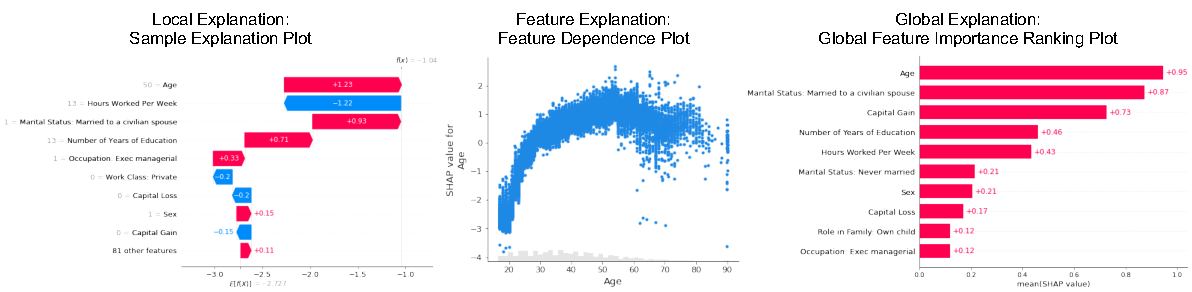
\includegraphics[width=\linewidth, bb=0 0 572 140]{figs/local_to_global.pdf}
    %\captionsetup{width=0.97\textwidth, aboveskip=5pt, belowskip=0pt, singlelinecheck=false}
    \caption{Explanations provided by the SHAP Python package. Left: A
      local explanation for a single data point. Each bar represents a
      single feature's attribution score for that data point. Middle:
      A single feature's attribution scores for all training data
      points, with each data point represented by a dot. Right:
      Global feature attributions obtained by taking the mean absolute
      value of each feature's absolute attribution scores across all
      training data points and then ranking the features by their
      average scores.}
    \label{fig:local_to_global}
\end{figure}

To explore whether ML developers would benefit from being able to
compare and contrast different global feature attributions, we ran an
artifact-based interview study with seven participants who had
experience with interpretability tools.  Participants were first shown
the usual global feature attributions provided by SHAP and asked some
questions about the underlying model.  They were then shown a suite of
global feature attributions obtained by ranking features by four
different summary statistics of their attribution scores---what we
refer to as a global feature attribution suite---and asked to
reconsider their answers.  We note that we do not view the global
feature attribution suite itself as a contribution, but rather as an
artifact for exploring ML developers' perceptions, needs, and
challenges around global feature attributions. Our study addresses the
following research questions:\looseness=-1
\begin{enumerate}
  \setlength\itemsep{0pt} \setlength\parskip{0pt} \item How do ML
  developers make sense of and use global feature attributions
  obtained by ranking features by different summary statistics of
  their attribution scores?
\item Does the ability to compare and contrast different global
  feature attributions allow ML developers to better understand the
  nuanced behavior of models?
\item What challenges do ML developers face when comparing and
  contrasting global feature attributions?
\end{enumerate}

We find that ML developers are able to use different global
feature attributions to achieve tasks and objectives including
communicating what their models have learned and identifying next
steps for debugging their models. Viewing the global feature
attribution suite increased participants' uncertainty in their
understanding of the underlying model (compared with viewing the usual
global feature attributions alone) as they became more aware of the
intricacies of the model's behavior. However, they expressed a tension
between the benefits obtained by using tools like SHAP to quickly get
a sense of what a model has learned and the time it would take to
compare and contrast different global feature attributions. This
tension might limit ML developers' willingness to use a global feature
attribution suite in their own workflows, echoing observations from
prior work about the need to balance the benefits of thinking fast and
thinking slow when designing interpretability
tools~\citep{InterpretingInterpretability}.\looseness=-1

This paper contributes to a recent line of research exploring
human-centered approaches to interpretability. Much of this research
focuses on how stakeholders use and understand interpretability tools
\citep{Lim, Bunt, Bussone, Hohman, Lage, Abdul, Hullman,
  InterpretingInterpretability, Zhang, Poursabzi-Sangdeh,AM21,VW21}.
Within this research, \citet{InterpretingInterpretability} found that
even experienced ML developers tend to misuse and place too much trust
in interpretability tools. They therefore suggested designing
interpretability tools that explicitly highlight the nuanced behavior
of models, as well as methods that counterbalance the bias toward
simple---and potentially misleading---explanations. We see our work as
a first exploration of how one might facilitate deeper understanding
by enhancing overly simplistic global views of a model.



\section{Preliminary Study}
\label{sec:phase1}

To better ground our research, we ran a small preliminary study during
the summer of 2020 to help us understand the current practices of
experienced users of interpretability tools. We conducted
semi-structured interviews with ten ML developers (e.g., data
scientists, research scientists, PhD students) across a variety of
domains (e.g., medicine, finance, retail). Participants were recruited
through a combination of posts to relevant email lists and message
boards at our institution, direct emails to individuals who had
written blog posts or made contributions to either the SHAP Python
package or InterpretML, and snowball sampling.  Each participant had
experience using at least one common interpretability tool, and nine
had experience specifically with SHAP.  Table~\ref{participantTable}
contains additional information about the participants.

During the interviews, we first asked participants about their
background and experience with both ML in general and interpretability
tools in particular. Next, we asked them to describe the
tasks and objectives they use interpretability tools to achieve, both
alone and with collaborators. Participants were asked to walk through
examples of specific times they had used interpretability tools to
accomplish those tasks and objectives, and were led through a series of
open-ended questions intended to uncover the strategies they had used,
including what had worked well and what had not.  Finally,
participants were asked if they had any wishes for a potential new
interpretability tool or for new functionality for an existing
interpretability tool. All interviews were conducted virtually on a
video conferencing platform due to the COVID-19 pandemic.  Audio from
the interviews was recorded and transcribed by a third-party service,
after which the audio transcripts were reviewed for accuracy and
anonymized. The first author then coded the transcripts using a
bottom-up approach and four authors conducted a thematic analysis. The
study was approved by our institution's IRB. Participation was
voluntary and participants received up to \$75 in compensation for
their participation.\footnote{Due to institutional requirements,
  compensation varied based on the relationship between the
  participant and our institution.}

\begin{table}[t!]
  \caption{Descriptions of the participants in our studies.}
  \label{participantTable}
  \begin{tabular}{llllll}
    \toprule
    \bf{ID} & \bf{Job Description} & \bf{\makecell[lt]{Years\\in ML}} & \bf{\makecell[lt]{Types of Data\\Worked With}} & \bf{\makecell[lt]{Interpretability Tools\\ or Methods Used}} & \bf{\makecell[lt]{Study 2\\Dataset}} \\
    \midrule
    P1 & ML PhD Student & 2 & Medical & \makecell[lt]{SHAP, self-made visualizations} & NHANES \\
\hline
    P2 & ML PhD Student & 1 & Medical & \makecell[lt]{InterpretML,
                                        SHAP, LIME, \\ GAMs, self-made visualizations} & NHANES \\
\hline
    P3 & ML Practitioner & 2 & \makecell[lt]{Remote Sensing,\\Retail,
    Banking} & \makecell[lt]{SHAP, self-made visualizations} & N/A \\
\hline
    P4 & \makecell[lt]{Environmental Sci.\\PhD Student}  & 3 & \makecell[lt]{Environmental,\\Geospatial} & \makecell[lt]{SHAP, GAMs,\\self-made visualizations} & N/A \\
\hline
    P5 & Data Scientist & 2 & Retail & SHAP & Adult \\  % P3 in other version
\hline
    P6 & \makecell[lt]{MD and ML PhD\\Student} & 4 & Medical & \makecell[lt]{SHAP, GAMs,\\self-made visualizations} & NHANES \\  % P4 in other version
\hline
    P7 & Research Scientist& 6 & \makecell[lt]{Technology,\\Medical} & \makecell[lt]{SHAP, LIME, GAMs,\\self-made visualizations} & Adult \\ % P5
\hline
    P8 & Data Scientist & 4 & Retail & AzureML, SHAP, LIME & Adult \\
    % P6
\hline
    P9 & \makecell[lt]{Data Scientist,\\Program Manager} & 7 & \makecell[lt]{Retail, Financial,\\User Behavior} & SHAP & N/A \\
\hline
    P10 & ML Practitioner & 3 & \makecell[lt]{Medical,\\Financial} & \makecell[lt]{InterpretML, AzureML, LIME,\\self-made visualizations} & Adult \\ % P7
    \bottomrule
  \end{tabular}
\end{table}

Participants described using interpretability tools for tasks and
objectives including model debugging, improving model performance,
communication and collaboration (including building collaborators'
trust in models), and knowledge discovery.  These tasks and objectives
are very much in line with those identified by \citet{Hullman}. In
total, participants mentioned more than forty different strategies for
accomplishing these tasks and objectives, such as looking for
patterns, outliers, and anomalies in scatter plots of feature
attribution scores for all training data points (as in the middle
panel of Figure \ref{fig:local_to_global}); comparing observed
patterns with prior knowledge; and turning to domain experts when some
aspect of an explanation was unclear.

Strikingly, although our preliminary study was not specifically
designed to explore the use of global feature attributions, all ten
participants said that they use global feature attributions (obtained using
the status quo approach of taking the mean absolute value of each
feature's attribution scores across all training data points and then
ranking the features by their average scores) somewhere in their
workflow.  Participants mentioned using global feature attributions to get an
overall sense of what their models have learned (e.g., for debugging
or for determining the overall credibility of their models), to check
that the ``most important'' features match their expectations, to
determine which features to prioritize for in-depth analysis, and to
communicate what their models have learned to other stakeholders.

However, participants also brought up several pain points around their
use of global feature attributions.  They were aware that using the mean
absolute value could be problematic.  As P2 said, \textit{``ranking of
  feature importance is, you know, a very-- somewhat arbitrary way to
  do things. You know, there's so many different importance
  measures. But, at least looking at something can tell us if our
  model has-- is relying on reasonable features.''}  Some participants
mentioned that using the mean absolute value fails to account for
relatively rare features that have a large influence when they are
present.  Participants also brought up the difficulty of communicating
about the global behavior of models at a level that is more in-depth
than the bar plots that common interpretability tools provide (see the
right panel of Figure \ref{fig:local_to_global}, for example).

Although it wasn't our original focus when we first set out to conduct
this preliminary study, observing participants' overwhelming use of
global feature attributions obtained using the status quo approach in their
workflows---despite being aware of some of the pitfalls---motivated us
to question whether ML developers would benefit from a more nuanced
global view of their models' behavior. That is the question we address
in this paper. Other needs that emerged from the study include ways to
explore and address feature correlation and confounding; less
time-consuming ways to analyze individual features; ways to aggregate
related features to understand their combined influence; ways to
determine the reliability of explanations; ways to validate insights
found using explanations; more customizable visualizations; and
increased documentation for interpretability tools, including
documentation aimed at expert users. We leave these directions for
future work. \looseness=-1





\section{Benefits and Drawbacks of Different Summary Statistics}
\label{sec:background}


In this section, we review the way in which global feature attributions are
most commonly obtained from feature attribution scores, describe some
alternative approaches to doing this, and discuss the benefits and
drawbacks of each. Although most of this discussion is applicable to
any local interpretability method that generates feature attribution
scores, we focus both here and in the rest of this paper on
SHAP~\citep{SHAP} for concreteness.  SHAP's feature attribution
scores, which are motivated by Shapley values from cooperative game
theory, can be viewed as a way of dividing the ``credit'' for a
model's prediction across all of its features.  The sum of the
features' attribution scores is equal to the expected value of the
prediction for the data point in question.  SHAP is widely used in
practice---as of November 2021, the SHAP Python package had close to
15k stars on GitHub, and nine of the ten participants in our
preliminary study had experience with SHAP.

We illustrate the benefits and drawbacks of different approaches to
obtaining global feature attributions from feature attribution scores through
case studies using models trained on two widely used open-source
datasets: the Adult dataset \citep{Adult} and the NHANES dataset
\citep{NHANES}. The Adult dataset is based on 1994 US Census data and
each data point corresponds to a person. The features include age,
employment type, education, marital status, occupation, race, and sex,
among others. The model that we trained on this dataset predicts
whether or not a person makes at least \$50k per year (the equivalent
of about \$92.5k in 2021 when adjusted for inflation). The NHANES
dataset is a survival dataset from a longitudinal health and wellness
study. Again, each data point corresponds to a person. The features
include age, race, sex, poverty index, BMI, lab blood test results,
and blood pressure measurements. The model that we trained on this
dataset is a Cox proportional hazards model that predicts the
differential risk of a person dying versus the typical background risk
(log hazard).

Although SHAP was designed to offer only local explanations, the SHAP
Python package additionally constructs makeshift global feature attributions as
follows: First, for each feature, take the mean absolute value of that
feature's attribution scores across all training data points. Next,
rank the features by their average scores. The resulting global
feature attributions for the models trained on the Adult and NHANES
datasets, respectively, can be seen in the top row of
Figure~\ref{fig:suite}.  For example, according to these global
feature attributions, age is the most important feature for both
models.  This is intuitive since people who are older tend to earn
more money and age is highly correlated with how likely someone is to
die in the near future. But this does not tell the whole story.  For
each of these models, does age play an equal role in the model's
predictions for all training data points, or is it more important for
some data points than for others?  Are there groups of data points for
which the model relies on completely different features?  Are there
outlier data points for which the model relies on features that it
should not?  If the goal is to debug the model, what should the next
step be?


\begin{figure}
    \centering
    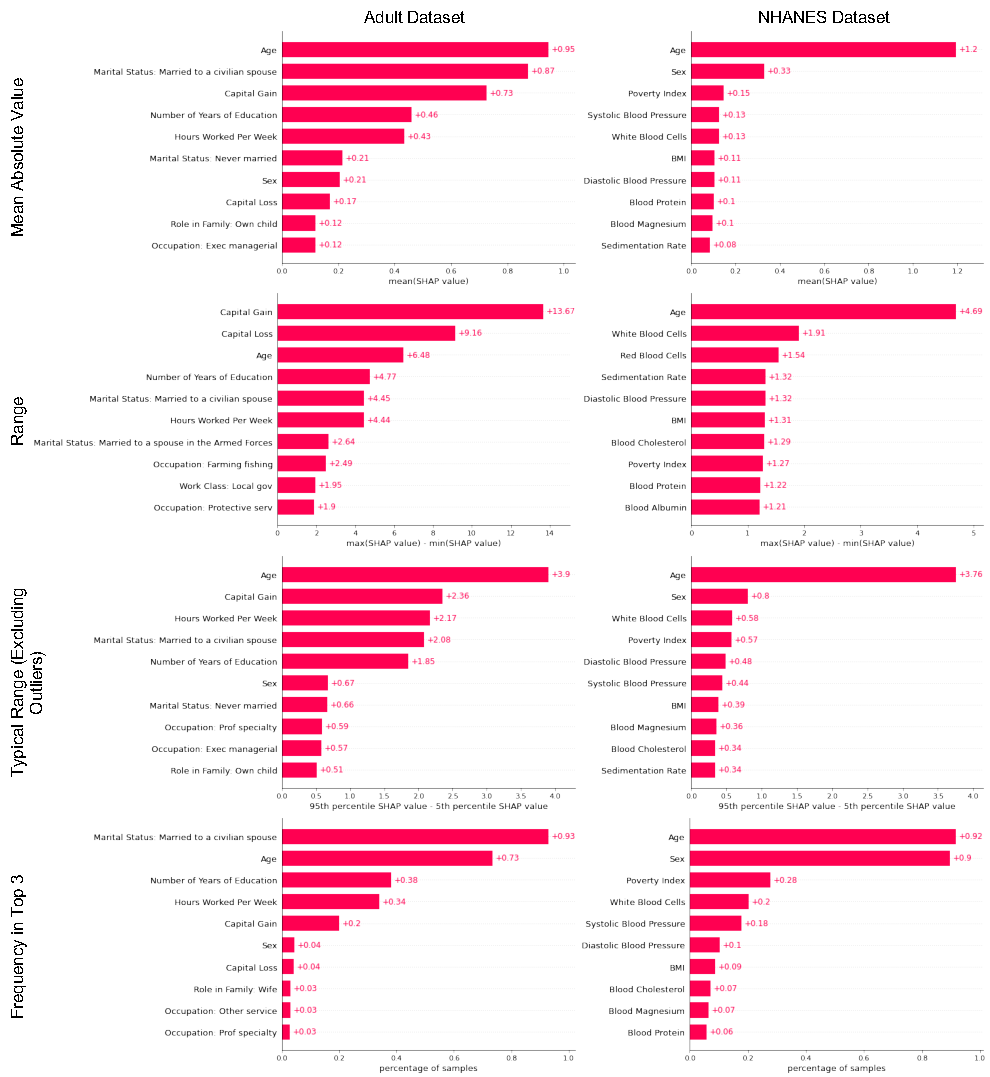
\includegraphics[width=\linewidth, bb=0 0 475 517]{figs/suite.pdf}
    \caption{Global feature attributions obtained by ranking features
      by different summary statistics of their attribution
      scores. Each row corresponds to a summary statistic: the mean
      absolute value, the range, the typical range, and the frequency
      in the top three.  The column on the left contains global
      feature attributions for the model trained on the Adult dataset;
      the column on the right contains global feature attributions for
      the model trained on the NHANES dataset.\looseness=-1}
    \label{fig:suite}
\end{figure}

To answer these questions, an ML developer could turn to a
visualization of a particular feature's attribution score across all
training data points, such as the type of scatter plot shown in the
middle panel of Figure \ref{fig:local_to_global} or the beeswarm plots
available in the SHAP Python package, both of which provide a more
detailed view of a feature's influence. However, for models with
hundreds or even thousands of features, it is too burdensome to
explore and compare all such plots---indeed, this is why developers
turn to summary statistics in the first place.  And even with a small
number of features, comparing plots across multiple features is not
easy.

Instead, we consider supplementing the mean absolute value with other
summary statistics. Using different summary statistics yields
different rankings of the features and, as we show below,
substantively different takeaways. Although in principle any summary
statistic could be used, we propose a few alternatives that capture
different aspects of the distribution of a model's feature attribution
scores across all training data points.\looseness=-1

We first consider the range of a feature's attribution scores---that
is, the difference between the maximum attribution score for that
feature across all training data points and the minimum attribution
score for that feature across all training data points (not taking
absolute values).  Features with a large range of attribution scores
are highly influential on at least some data points.  Outlier data
points can be found by examining scatter plots for features with a
large range.  This is useful both for understanding a model's behavior
on unusual data points and for identifying bugs.  As we can see from
the second row of Figure~\ref{fig:suite}, when predicting whether
someone makes over \$50k a year using the Adult dataset, capital loss
is only the eighth-highest ranked feature when using the mean absolute
value, but the second-highest ranked feature in terms of range. This
is due to extreme outliers---specifically, atypically high capital
loss values---in the training dataset. The prominence of capital loss
in this alternative ranking might help draw a developer's attention to
this issue so they can investigate whether it stems from a bug that
needs fixing or whether it reflects a true phenomenon in the
underlying population.\looseness=-1

In some cases, the range may be too susceptible to outliers. Even a
single data point with an extreme feature attribution score can boost
a feature's range.  This can be problematic if the goal is not to
identify individual outlier data points, but to identify larger groups
of data points for which a feature is highly influential.  As a
result, for this task, it may be more appropriate to use a censored
version of the range.  We define the typical range of a feature's
attribution scores to be the difference between the feature's
ninety-fifth-percentile feature attribution score and its fifth
percentile feature attribution score across all training data
points.\footnote{The choice of the ninety-fifth percentile and the
  fifth percentile is, of course, somewhat arbitrary, and other
  percentiles could be used; we thought that this choice would balance
  the ability to identify groups of data points with robustness to
  extreme outliers.} Ranking features by their typical range can
reveal features that are influential not just for a handful of data
points, but for a more substantial subset of data points. It can
therefore be used to identify groups of data points for which the
model behaves similarly. Examining the second row of
Figure~\ref{fig:suite}, we can see that both red blood cell count and
white blood cell count have a large range for the NHANES model.
However, examining the third row, we can see that only white blood
cell count ranks highly in terms of the typical range. This suggests
that white blood cell count is an important feature for a larger
subset of the training data points than red blood cell count, for
which the large range may be due to outliers.\looseness=-1


The final summary statistic that we consider enables us to get a sense
of which features are influential for a large proportion of the
training data points without worrying about the specific values of
their attribution scores.  We define the frequency in the top three to
be the fraction of the training data points for which the feature in
question ranks among the top three in terms of its absolute feature
attribution scores.  We can think of this as letting every data point
vote for its top three most important features and then tallying up
the votes across the training dataset.\footnote{Again, the choice of
  three votes per data point is arbitrary and other values could be
  used.}  Compared with the mean absolute value, the frequency in the
top three provides a way to control for high variance in the feature
attribution scores.  When predicting whether someone will make over
\$50k a year using the Adult Dataset, the capital gain feature ranks
third in terms of the mean absolute value, and one might therefore
assume it is important for all data points.  However, examining the
final row of Figure~\ref{fig:suite}, we can see that capital gain is
one of the top three most important features for only 20\% of the
training data points. In contrast, hours worked per week is in the top
three for 34\% of the training data points, while its mean absolute
feature attribution score is significantly lower (0.43, compared with
0.73 for capital gain).\looseness=-1


Different summary statistics will yield different global feature attributions
that can be used to derive different---and often
complementary---insights.  We therefore propose that a more accurate
global view of a model's behavior might be achieved by allowing ML
developers to compare and contrast different global feature attributions. In
the next section, we describe a study that we designed to explore this
idea.\looseness=-1


\section{Main Study}

To explore whether ML developers would benefit from being able to
compare and contrast different global feature attributions, we ran a
study in which participants were asked to answer questions about a
model before and after seeing global feature attributions obtained by
ranking features by four different summary statistics of their
attribution scores, as described in Section~\ref{sec:background}. We
refer to this as a global feature
attribution suite, and use it as an artifact for exploring ML
developers' perceptions, needs, and challenges around global feature
attributions.\looseness=-1

\subsection{Methods}

For this study, which we conducted during the summer of 2020, we
recruited seven participants, all of whom had participated in our
preliminary study (see Section~\ref{sec:phase1}) and had agreed to be
contacted for follow-up research; the remaining three participants
declined to participate. The study was approved by our institution's
IRB. Each interview lasted approximately one hour and participants
received a \$50 gift card for their participation.

The study consisted of semi-structured interviews in which
participants were shown two different static (HTML file) Jupyter
notebooks.  Both notebooks contained a model, a textual description of
the dataset used to train the model, a beeswarm plot visualizing the
distribution of attribution scores for each feature, and a feature
dependence scatter plot for each feature (as in the middle panel of
Figure \ref{fig:local_to_global}). In the first notebook, we included
a bar plot showing global feature attributions obtained using the
status quo approach---that is, by taking the mean absolute value of
each feature's attribution scores across all training data points and
then ranking the features by their average scores, as in the top row
of Figure~\ref{fig:suite}---as well as a description of how these
global feature attributions were obtained and a brief list of
potential uses. In the second notebook, we additionally included bar
plots showing global feature attributions obtained using other summary
statistics (specifically, the range, the typical range, and the
frequency in the top three) in addition to the mean absolute value, as
shown in Figure~\ref{fig:suite}. We described how these global feature
attributions were obtained and listed potential uses for each, using
the wording in Table~\ref{tab:descriptions}. All participants were
shown the first notebook before the second notebook. We chose to show
the notebooks sequentially, as opposed to using a counterbalanced
design, so that we could first observe how participants made use of
the usual global feature attributions provided by SHAP, and then see
whether and how their perspectives changed when they were shown the
global feature attribution suite.

\begin{table}[t!]
  \caption{The descriptions of the summary statistics that were shown to participants.}
  \label{tab:descriptions}
  \begin{tabular}{p{0.1\linewidth} p{0.35\linewidth} p{0.47\linewidth}}
    \toprule
    \bf{Statistic} & \bf{How It's Calculated} & \bf{Potential Uses} \\
    \midrule
    Mean Absolute Value & Mean over all samples in the training data set of the absolute value of each sample's model attribution score. & Gives a sense of what the model is learning overall. Currently the default global feature importance ranking in SHAP. \\
\hline
    Range &  Difference between the maximum model attribution score and the minimum model attribution score of the given feature over the training data set. & Identifies features that are heavily influential on at least a small number of samples in the data. Can also help find extreme outliers in the data. \\
\hline
    Typical Range (Excluding Outliers) & Difference between the 95th percentile model attribution score and the 5th percentile model attribution score of the given feature over the training data set. & Identifies features that are heavily influential for at least a substantial subset of samples within the data. More robust to outliers than the Range. Can also help find subsets within the data. \\
\hline
    Frequency in the Top Three & Fraction of samples in the training data set for which the given feature was ranked in the top three in terms of absolute attribution scores.  & Gives a sense of which features most commonly have heavy influence on individual samples' predictions. Can also help to get an understanding without needing to understand the model attribution score. \\
    \bottomrule
  \end{tabular}
\end{table}

To avoid over-indexing on a single dataset or model, we generated
versions of these notebooks for both of the models described in
Section~\ref{sec:background}---that is, the model trained on the Adult
dataset and the model trained on the NHANES dataset.  We assigned the
model trained on the NHANES dataset to the three participants who most
regularly work with medical data and would therefore likely be more
comfortable with both the task and the features; we assigned the model
trained on the Adult dataset to the remaining four participants.
These assignments are listed in the rightmost column of
Table~\ref{participantTable}.

All interviews were conducted virtually on a video conferencing
platform due to the COVID-19 pandemic.  During each interview, the
participant and the interviewer viewed the notebooks together, one at
a time, via screen sharing. The participant had control of the screen
to click, scroll, and explore. Participants were first asked to think
aloud while they familiarized themselves with each notebook. They were
then asked how they would go about accomplishing three of the tasks
and objectives for which participants in our preliminary study had
reported using interpretability tools. Specifically, we asked
participants to describe 1) what they thought the model had learned
overall, 2) how they would explain what the model had learned to
someone who wasn't an ML developer, and 3) what their next steps would
be if they were to go about debugging the model. After completing this
sequence with the first notebook, and then completing it again with
the additional information provided in the second notebook,
participants were asked to share their likes and dislikes for each of
the different global feature attributions, as well as their critical
feedback, the value they gained from using the global feature
attribution suite, and whether they would use a global feature
attribution suite in their own workflows.  The complete notebooks and
the interview protocol can be found at
\url{https://github.com/aokeson/Aggregated-Explainability-Ranking-Alternatives}.

Both audio and video from the interviews was recorded.  Audio was
transcribed by a third-party service, after which the audio
transcripts were reviewed for accuracy and anonymized.  The first
author then annotated each transcript with information about the
visualizations that the participant viewed at different points in time
based on the corresponding video recording. The annotated transcripts
were coded by the first author in three distinct passes: 1) coding
differences in how participants answered our questions when viewing
the first notebook compared with the second notebook, 2) coding
potential uses mentioned by participants for the different global
feature attributions, and finally 3) coding feedback (both positive
and negative) on the global feature attribution suite. All authors
then participated in a thematic analysis using the three types of
codes.

\subsection{Results}
As we describe in this section, participants found the global feature
attribution suite useful for communicating what the model had learned
and identifying next steps for debugging the model. They also found
that it increased their uncertainty in their understanding the model
(compared with viewing the usual global feature attributions alone)
and helped them become more aware of the nuances of the model's
behavior. However, they expressed concerns that the time it would take
to compare and contrast different global feature attributions might
affect the extent to which they would use a global feature attribution
suite in their own workflows.

With our small sample size, we did not see clear differences between
participants who were shown the model trained on the NHANES dataset
and participants who were shown the model trained on the Adult
datasets, so we do not attempt to make distinctions between the two.

\subsubsection{Strategies for Using Different Global Feature Attributions}
Participants used the global feature attributions in a variety of
different ways, exploring them individually as well as comparing and
contrasting different global feature attributions.

Three participants (P5, P6, P7) checked for agreement between the
different global feature attributions in order to pull out specific
features that were influential across more than one of them. This gave
them more confidence that these features were genuinely
influential. For example, P5, who saw the model trained on the Adult
dataset, had named age as being important to the model's predictions
when they viewed the usual global feature attributions provided by
SHAP in the first notebook. After seeing that age was also highly
ranked according to the global feature attributions provided in the
second notebook, they were more confident in their assessment of what
the model had learned and in how to communicate what the model had
learned to other stakeholders, stating \textit{``I would feel rather
  confident that the clearest learning from the model is [...]  around
  age.''} P6 and P7 both independently described this process as
trying to ``flatten'' the different global feature attributions back
to a single list of the most influential features by extracting
features that were highly ranked according to all of the global
feature attributions. \textit{``Maybe you want to start by listing the
  features that are sort of robustly important across an array of
  these different metrics.''} --P6 \looseness=-1

One of the most common strategies for using the global feature
attribution suite was to identify where the different global feature
attributions disagreed and to explore the cause of this
disagreement. Five of the seven participants (P1, P2, P6, P7, and P8)
discussed using this strategy either to uncover new insights into the
model's predictions or as a first step for debugging the model. P7
described going through each feature to check if it was consistently
important, unimportant, or both across the different global feature
attributions: \textit{``Consistently important variables,
  great. Consistently not important variables, great. But variables
  where some trick like that could move you around a lot maybe is
  indicating something. Exactly what, I don't know. But that's why I
  would have to go explore.''} As P6 described, \textit{``It seems
  potentially very useful to come up with several different orderings
  of the features and then try to figure out why those orderings
  disagree in cases where they disagree. That seems like a very
  potentially fruitful way to find either interesting behavior or
  problems with your model.''}  P8, who saw the model trained on the
Adult dataset, also used this strategy.  When looking at the first
notebook, P8 included capital gain in a list of influential features,
because it was among the top three features according to the global
feature attributions obtained using the status quo approach. However,
while exploring the second notebook, P8 found that the different
global feature attributions differed in their rankings of capital gain
and capital loss, and decided to explore this further. They were able
to use this observation to jump start the debugging process by
identifying outliers in the training dataset: \textit{``I think that
  probably the [range] or [typical range] here helps to explain why
  capital gains appears on the [ranking by mean absolute value] but
  rather not in the [ranking by frequency in top three], probably
  because [capital gains] has very high variance and there are some
  outliers in the data, which drags this mean absolute value here. So,
  the outliers are the main cause that drag this capital gain to be
  the top three in [ranking by mean], rather than the [ranking by
    frequency in the top three].''} \looseness=-1

There was no general consensus among participants about which of the
global feature attributions was most appropriate for each of the three
tasks and objectives.  In general, participants followed the brief
guidance that we had provided in the notebooks about potential uses.
For example, P2, who saw the model trained on the NHANES dataset, used
the global feature attributions obtained by ranking features by their
range to identify outliers in the training dataset, saying
\textit{``This range of the blood cell value, so I would want to
  verify that that's a realistic effect, that we're not just picking
  up individuals that have bad values for the white blood cell
  count.''}  In some cases, participants also came up with their own
uses for the different global feature attributions, either
deliberately or by chance. P2, for example, identified a potential bug
in the NHANES dataset after examining the global feature attributions
obtained by ranking features by their frequency in the top three and
then deciding to dig more deeply into the diastolic blood pressure
feature.  \textit{``For instance, there is a group of patients here
  with diastolic blood pressure less than 20. That hardly seems
  realistic. So this is a group of patients for whom either the value
  is missing or it was input wrong.''} --P2

\subsubsection{Increased Uncertainty about the Model's Behavior}

Our hope was that providing ML developers with different global
feature attributions to compare and contrast would lessen their
confidence in the overly simplistic global feature attributions
usually provided by SHAP and instead enable them to obtain a more
nuanced global view of their models' behavior. When interacting with
the first notebook, most participants focused their descriptions of
what the model had learned on a few features that were highly ranked
according to the usual global feature attributions provided by
SHAP. As a result, participants tended to focus their exploration of
the model on a few (typically three to five) features. However, when
exploring the second notebook, participants began to doubt the simple
answers they had given previously.  For example, P7 questioned their
initial interpretation of what the model had learned, saying
\textit{``Now I'm a little hesitant, because I'm not sure. I guess
  there's now four plots, and they are kind of equivalent. [...] So
  now I'm a little confused. I'm not sure which one to trust and to
  use to answer this question.''}  Participants also commented that
their confidence had changed: \textit{``I think it's just sort of
  broadened my confidence intervals on how important each feature
  is.''} \hbox{--P6}.  As desired, participants felt that the global
feature attribution suite provided a more nuanced global view of the
model's behavior than the global feature attributions obtained using
the status-quo approach: \textit{``I mean, it takes you from [...] a
  scalar importance to a distribution of importance. It really helps
  you get that new understanding of how the importance of a feature
  can change over the different samples and the mean will not tell you
  that.''}  --P2 Lastly, participants noted that some of the
information available in the second notebook could be inferred from
other visualizations, such as SHAP's beeswarm plots, but that the new
plots made it easier to digest and interpret the information:
\textit{``I mean, that's similar information for what's in this
  summary plot, but it's condensed in a way that it's much easier to
  read.''} --P2 Indeed, although the distribution of attribution
scores for each feature was available in other plots, this information
was not salient enough to mitigate participants'
overconfidence.\looseness=-1

\subsubsection{Required time investment and constraints} \label{sec:time_investment}

The most common challenge raised by participants was that it might be
too time consuming to compare and contrast different global feature
attributions. P7 articulated a tension between the pressures of
real-world time constraints and the benefits of rigorously examining
multiple global feature attributions: \textit{``And if you are really
  strapped for time, which in the industry you frequently are, then it
  might be easy to just not explore these other things. [...] It makes
  me think that, going forward, I should be a little more vigilant
  about this stuff, but, honestly, it really depends on time.''}
Participants were concerned about whether a global feature attribution
suite would help them accomplish their tasks and objectives more
quickly or instead be yet another time sink.  Participants may have
been overly pessimistic about the time it would take to compare and
contrast different global feature attributions because they were
seeing them for the first time. However, before implementing a global
feature attribution suite in common interpretability tools, more
research is needed to understand how to present different global
feature attributions in the most efficient way possible.

\section{Discussion}

We presented an artifact-based interview study intended to investigate
whether ML developers would benefit from being able to compare and
contrast different global feature attributions. This study extends a
recent line of research exploring human-centered approaches to
interpretability and, in particular, how stakeholders use and
understand interpretability tools~\citep{Lim, Bunt, Bussone, Hohman,
  Lage, Abdul, Hullman, InterpretingInterpretability, Zhang,
  Poursabzi-Sangdeh,AM21,VW21}; however, our focus is on an aspect of
interpretability tools that has been overlooked to date---namely, the
summary statistics used to generate global feature
attributions. Participants were first shown the usual global feature
attributions provided by SHAP and asked some questions about the
underlying model. They were then shown a suite of global feature
attributions obtained by ranking features by four different summary
statistics of their attribution scores---what we refer to as a global
feature attribution suite---and asked to reconsider their answers. Our
hope was that providing ML developers with different global feature
attributions to compare and contrast would lessen their confidence in
the overly simplistic global feature attributions usually provided by
SHAP and instead enable them to obtain a more nuanced global view of
their models' behavior.\looseness=-1

We found that participants were able to use the global feature
attribution suite to communicate what the model had learned and to
identify next steps for debugging the model. As desired, we also found
that viewing the global feature attribution suite increased their
uncertainty in their understanding of the underlying model as they
became more aware of the intricacies of the model's behavior. However,
they also expressed a tension between the benefits obtained by using
tools like SHAP to quickly get a sense of what a model has learned and
the time it would take to compare and contrast different global
feature attributions, noting that this might affect the extent to
which they would use a global feature attribution suite in their own
workflows. Of course, participants were seeing the global feature
attributions for the first time and they only used the global feature
attribution suite for less than an hour. It is possible that with
adequate training and practice, this tension would be reduced or even
overcome. Longitudinal studies may be beneficial for investigating
further. More generally, though, this finding echoes observations from
prior work about the need to balance the benefits of thinking fast and
thinking slow when designing interpretability
tools~\citep{InterpretingInterpretability}.

Like any study, ours has limitations. In addition to the short
timescale over which it was conducted, we only recruited seven
participants. We wanted to be able to conduct an in-depth interview
with each participant about their experiences using the global feature
attribution suite, but this necessarily limits the type of conclusions
that we are able to draw. Furthermore, we focused only on experienced
users of interpretability tools, which further limits the extent to
which we can generalize to the broader ML developer community.  We
also limited our scope to models trained on two datasets, so more
research is needed to investigate whether our findings would change if
different datasets were used---for example, datasets with orders of
magnitude more features. \looseness=-1

We see our work as a first step toward designing interpretability
tools that explicitly highlight the nuanced behavior of models, as
advocated for by \citet{InterpretingInterpretability}. Future work
should explore ways for ML developers to use a global feature
attribution suite to quickly get a sense of what a model has learned
without placing undue confidence in the corresponding global feature
attributions. This will require carefully balancing the cognitive
burden involved in understanding the global feature attributions with
the amount of information that they can convey. It will also require
investigation into which summary statistics to use and which other
information to incorporate. One could imagine, for example,
additionally including other notions of global feature importance,
such as those obtained by applying the concept of Shapley values
directly to global quantities like the variance explained~\citep{OP17}
and the loss~\citep{CLL20} rather than summarizing (local) feature
attribution scores. Doing this well will also require research into
how to present different global feature attributions in the most
efficient way possible.




\section*{Acknowledgments}
We are grateful to members of Microsoft's FATE group and the
  Aether Transparency Working Group---especially Mehrnoosh
  Sameki---for valuable discussions and feedback.


\begin{thebibliography}{10}
\itemsep=1pt
\begin{small}


\bibitem[Abdul et~al.(2020)Abdul, von~der Weth, Kankanhalli, and Lim]{Abdul}
A.~Abdul, C.~von~der Weth, M.~Kankanhalli, and B.~Y. Lim.
\newblock {COGAM}: {M}easuring and moderating cognitive load in machine
  learning model explanations.
\newblock In \emph{Proceedings of the 2020 CHI Conference on Human Factors in Computing
  Systems}, 2020.

\bibitem[Alvarez-Melis et~al.(2021)Alvarez-Melis, Kaur, {Daum\'e III}, Wallach,
  and Vaughan]{AM21}
D.~Alvarez-Melis, H.~Kaur, H.~{Daum\'e III}, H.~Wallach, and J.~W. Vaughan.
\newblock From human explanation to model interpretability: {A} framework based
  on weight of evidence.
\newblock In \emph{AAAI Conference on Human Computation and Crowdsourcing
  (HCOMP)}, 2021.

\bibitem[Barocas et~al.(2021)Barocas, Guo, Kamar, Krones, Morris, Vaughan,
  Wadsworth, and Wallach]{BG+21}
S.~Barocas, A.~Guo, E.~Kamar, J.~Krones, M.~R. Morris, J.~W. Vaughan,
  D.~Wadsworth, and H.~Wallach.
\newblock Designing disaggregated evaluations of ai systems: {C}hoices,
  considerations, and tradeoffs.
\newblock In \emph{Proceedings of the Fourth AAAI/ACM Conference on Artificial
  Intelligence, Ethics, and Society (AIES)}, 2021.

\bibitem[Bunt et~al.(2012)Bunt, Lount, and Lauzon]{Bunt}
A.~Bunt, M.~Lount, and C.~Lauzon.
\newblock Are explanations always important? {A} study of deployed, low-cost
  intelligent interactive systems.
\newblock In \emph{Proceedings of the 2012 ACM International Conference on
  Intelligent User Interfaces}, 2012.

\bibitem[Bussone et~al.(2015)Bussone, Stumpf, and O'Sullivan]{Bussone}
A.~Bussone, S.~Stumpf, and D.~O'Sullivan.
\newblock The role of explanations on trust and reliance in clinical decision
  support systems.
\newblock In \emph{2015 International Conference on Healthcare Informatics},
  2015.

\bibitem[Caruana et~al.(2015)Caruana, Lou, Gehrke, Koch, Sturm, and
  Elhadad]{Caruana2015-qf}
R.~Caruana, Y.~Lou, J.~Gehrke, P.~Koch, M.~Sturm, and N.~Elhadad.
\newblock Intelligible models for {HealthCare} : Predicting pneumonia risk and
  hospital 30-day readmission.
\newblock In \emph{Proceedings of the 21th ACM SIGKDD International Conference
  on Knowledge Discovery and Data Mining}, 2015.

\bibitem[{Centers for Disease Control and Prevention}(1974)]{NHANES}
{Centers for Disease Control and Prevention}.
\newblock {NHANES} data set, 1974.
\newblock Data retrieved from SHAP python package,
  \url{https://github.com/slundberg/shap/tree/master/data}.

\bibitem[Covert et~al.(2020)Covert, Lundberg, and Lee]{CLL20}
I.~Covert, S.~Lundberg, and S.-I. Lee.
\newblock Understanding global feature contributions with additive importance
  measures.
\newblock In \emph{Advances in Neural Information Processing Systems 33}, 2020.

\bibitem[Hastie and Tibshirani(1990)]{hastie1990generalized}
T.~J. Hastie and R.~J. Tibshirani.
\newblock \emph{Generalized Additive Models}.
\newblock CRC Press, June 1990.

\bibitem[Hohman et~al.(2019)Hohman, Head, Caruana, DeLine, and Drucker]{Hohman}
F.~Hohman, A.~Head, R.~Caruana, R.~DeLine, and S.~M. Drucker.
\newblock Gamut: A design probe to understand how data scientists understand
  machine learning models.
\newblock In \emph{Proceedings of the 2019 CHI Conference on Human Factors in Computing
  Systems}, 2019.

\bibitem[Hong et~al.(2020)Hong, Hullman, and Bertini]{Hullman}
S.~R. Hong, J.~Hullman, and E.~Bertini.
\newblock Human factors in model interpretability: Industry practices,
  challenges, and needs.
\newblock \emph{Proceedings ACM Human-Computer Interaction}, 4\penalty0 (CSCW1), 2020.

\bibitem[Jung et~al.(2020)Jung, Concannon, Shroff, Goel, and
  Goldstein]{jung2020simple}
J.~Jung, C.~Concannon, R.~Shroff, S.~Goel, and D.~G. Goldstein.
\newblock Simple rules to guide expert classifications.
\newblock \emph{Journal of the Royal Statistical Society: Series A (Statistics
  in Society)}, 183\penalty0 (3):\penalty0 771--800, 2020.

\bibitem[Kaur et~al.(2020)Kaur, Nori, Jenkins, Caruana, Wallach, and
  Wortman~Vaughan]{InterpretingInterpretability}
H.~Kaur, H.~Nori, S.~Jenkins, R.~Caruana, H.~Wallach, and J.~Wortman~Vaughan.
\newblock Interpreting interpretability: Understanding data scientists’ use
  of interpretability tools for machine learning.
\newblock In \emph{Proceedings of the 2020 CHI Conference on Human Factors in
  Computing Systems}, 2020.

\bibitem[Koh and Liang(2017)]{KL17}
P.~W. Koh and P.~Liang.
\newblock Understanding black-box predictions via influence functions.
\newblock In \emph{Proceedings of the 34th International Conference on Machine
  Learning ({ICML})}, 2017.

\bibitem[Kohavi and Becker(1996)]{Adult}
R.~Kohavi and B.~Becker.
\newblock Adult data set, 1996.
\newblock Data retrieved from SHAP python package,
  \url{https://github.com/slundberg/shap/tree/master/data}.

\bibitem[Lage et~al.(2019)Lage, Chen, He, Narayanan, Kim, Gershman, and
  Doshi-Velez]{Lage}
I.~Lage, E.~Chen, J.~He, M.~Narayanan, B.~Kim, S.~J. Gershman, and
  F.~Doshi-Velez.
\newblock Human evaluation of models built for interpretability.
\newblock In \emph{AAAI Conference on Human Computation and Crowdsourcing
  (HCOMP)}, 2019.

\bibitem[Lim and Dey(2011)]{Lim}
B.~Y. Lim and A.~K. Dey.
\newblock Investigating intelligibility for uncertain context-aware
  applications.
\newblock In \emph{Proceedings of the 13th International Conference on
  Ubiquitous Computing}, 2011.

\bibitem[Lundberg and Lee(2017)]{SHAP}
S.~M. Lundberg and S.-I. Lee.
\newblock A unified approach to interpreting model predictions.
\newblock In \emph{Advances in Neural Information Processing Systems 30}, 2017.

\bibitem[Nushi et~al.(2018)Nushi, Kamar, and Horvitz]{Nushi2018}
B.~Nushi, E.~Kamar, and E.~Horvitz.
\newblock Towards accountable {AI}: {H}ybrid human-machine analyses for
  characterizing system failure.
\newblock In \emph{AAAI Conference on Human Computation and Crowdsourcing
  (HCOMP)}, 2018.

\bibitem[Owen and Prieur(2017)]{OP17}
A.~B. Owen and C.~Prieur.
\newblock On {S}hapley value for measuring importance of dependent inputs.
\newblock \emph{SIAM/ASA Journal on Uncertainty Quantification}, 51\penalty0 (1):\penalty0 986--1002, 2017.

\bibitem[Poursabzi-Sangdeh et~al.(2021)Poursabzi-Sangdeh, Goldstein, Hofman,
  Wortman~Vaughan, and Wallach]{Poursabzi-Sangdeh}
F.~Poursabzi-Sangdeh, D.~G. Goldstein, J.~M. Hofman, J.~W. Wortman~Vaughan, and
  H.~Wallach.
\newblock Manipulating and measuring model interpretability.
\newblock In \emph{Proceedings of the 2021 CHI Conference on Human Factors in Computing
  Systems}, 2021.

\bibitem[Quinlan(1986)]{quinlan1986induction}
J.~R. Quinlan.
\newblock Induction of decision trees.
\newblock \emph{Maching Learning}, 1\penalty0 (1):\penalty0 81--106, 1986.

\bibitem[Ribeiro et~al.(2016)Ribeiro, Singh, and Guestrin]{LIME}
M.~T. Ribeiro, S.~Singh, and C.~Guestrin.
\newblock "{W}hy should {I} trust you?": {E}xplaining the predictions of any
  classifier.
\newblock In \emph{Proceedings of the 22nd {ACM} {SIGKDD} International
  Conference on Knowledge Discovery and Data Mining}, 2016.

\bibitem[Robinson(1950)]{R50}
W.~S. Robinson.
\newblock Ecological correlations and the behavior of individuals.
\newblock \emph{American Sociological Review}, 15\penalty0 (3):\penalty0
  351--357, 1950.

\bibitem[Rudin(2019)]{rudin2019please}
C.~Rudin.
\newblock Stop explaining black box machine learning models for high stakes
  decisions and use interpretable models instead.
\newblock \emph{Nature Machine Intelligence}, 1\penalty0 (5):\penalty0
  206--215, 2019.

\bibitem[Russell(2019)]{R19b}
C.~Russell.
\newblock Efficient search for diverse coherent explanations.
\newblock In \emph{Proceedings of the Conference on Fairness, Accountability,
  and Transparency ({FAT*})}, 2019.

\bibitem[Ustun et~al.(2019)Ustun, Spangher, and Liu]{USL19}
B.~Ustun, A.~Spangher, and Y.~Liu.
\newblock Actionable recourse in linear classification.
\newblock In \emph{Proceedings of the Conference on Fairness, Accountability,
  and Transparency ({FAT*})}, 2019.

\bibitem[Vaughan and Wallach(2021)]{VW21}
J.~W. Vaughan and H.~Wallach.
\newblock A human-centered agenda for intelligible machine learning.
\newblock In M.~Pelillo and T.~Scantamburlo, editors, \emph{Machines We Trust:
  Perspectives on Dependable AI}. MIT Press, 2021.

\bibitem[Weld and Bansal(2019)]{WB19}
D.~S. Weld and G.~Bansal.
\newblock The challenge of crafting intelligible intelligence.
\newblock \emph{Comm. of the ACM}, 62\penalty0 (6):\penalty0 70--79, 2019.

\bibitem[Zeng et~al.(2017)Zeng, Ustun, and Rudin]{zeng2017interpretable}
J.~Zeng, B.~Ustun, and C.~Rudin.
\newblock Interpretable classification models for recidivism prediction.
\newblock \emph{Journal of the Royal Statistical Society: Series A (Statistics
  in Society)}, 180\penalty0 (3):\penalty0 689--722, 2017.

\bibitem[Zhang et~al.(2020)Zhang, Muller, and Wang]{Zhang}
A.~X. Zhang, M.~Muller, and D.~Wang.
\newblock How do data science workers collaborate? {R}oles, workflows, and
  tools.
\newblock \emph{Proceedings ACM Human-Computer Interaction}, 4\penalty0 (CSCW1), 2020.


\end{small}
\end{thebibliography}


%\bibliographystyle{abbrvnat}
%{\small
%\bibliography{bib}
%}


\end{document}
